\documentclass[tikz]{standalone}
\usepackage{times}
\usepackage{amsmath}
\usepackage{txfonts}
\usepackage[utf8]{inputenc}
\usepackage{graphics}
\usepackage{pgfplots}
\usetikzlibrary{arrows,intersections,math}
\usetikzlibrary{patterns}
\usetikzlibrary{pgfplots.fillbetween}
\usepackage{ifthen}
\begin{document}
	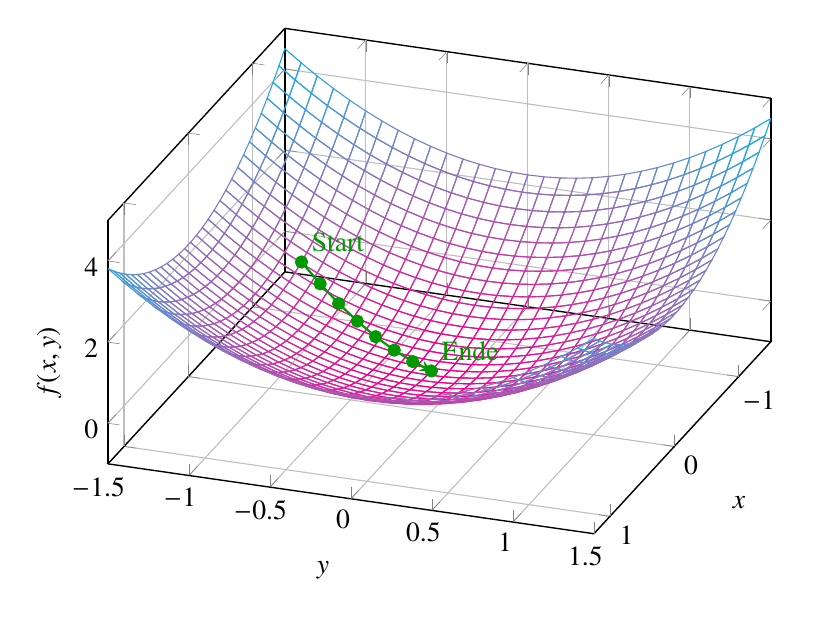
\begin{tikzpicture}
		\definecolor{drkGrenn}{rgb}{0.0, 0.6, 0.0}
		\begin{axis}[
			width=10cm,
			height=8cm,
			view={110}{40},
			grid=major,
			xlabel={$x$},
			ylabel={$y$},
			zlabel={$f(x,y)$},
			axis line style = {line width=0.5pt},
			zmin=-1,
			zmax=5,
			domain=-1.5:1.25,
			y domain=-1.5:1.5,
			colormap={invertedcool}{color(0cm)=(magenta); color(0.5cm)=(cyan)},
			]
			\addplot3[
			mesh,
			shader=interp,
			samples=31,
			domain=-1.5:1.25,
			y domain=-1.5:1.5
			] {x^2 + y^2};
			
			\addplot3[
			thick,
			drkGrenn,
			mark=*,
			mark options={solid},
			-stealth,
			line join=bevel,
			point meta=explicit symbolic,
			nodes near coords={
				\ifdim\coordindex pt=0pt Start\fi
				\ifdim\coordindex pt=7pt Ende\fi
			},
			every node near coord/.append style={anchor=south west, color=drkGrenn}
			] coordinates {
				(-0.5, -1, 1.25)   
				(-0.429, -0.857, 0.918)
				(-0.357, -0.714, 0.638)
				(-0.286, -0.571, 0.408)
				(-0.214, -0.429, 0.230)
				(-0.143, -0.286, 0.102)
				(-0.071, -0.143, 0.026)
				(0, 0, 0)      
			};
		\end{axis}
	\end{tikzpicture}
\end{document}

